\documentclass{article}


\usepackage{arxiv}

\usepackage[utf8]{inputenc} % allow utf-8 input
\usepackage[T1]{fontenc}    % use 8-bit T1 fonts
\usepackage{hyperref}       % hyperlinks
\usepackage{url}            % simple URL typesetting
\usepackage{booktabs}       % professional-quality tables
\usepackage{amsfonts}       % blackboard math symbols
\usepackage{nicefrac}       % compact symbols for 1/2, etc.
\usepackage{microtype}      % microtypography
\usepackage{lipsum}
\usepackage{todonotes}

\title{Monitoring the Growth of Mangroves using Camera Images}


\author{
  Q. Xiang\thanks{Use footnote for providing further
    information about author (webpage, alternative
    address)---\emph{not} for acknowledging funding agencies.} \\
  Department of Computer Science\\
  Cranberry-Lemon University\\
  Pittsburgh, PA 15213 \\
  \texttt{hippo@cs.cranberry-lemon.edu} \\
  %% examples of more authors
   \And
 Elias D.~Striatum \\
  Department of Electrical Engineering\\
  Mount-Sheikh University\\
  Santa Narimana, Levand \\
  \texttt{stariate@ee.mount-sheikh.edu} \\
  %% \AND
  %% Coauthor \\
  %% Affiliation \\
  %% Address \\
  %% \texttt{email} \\
  %% \And
  %% Coauthor \\
  %% Affiliation \\
  %% Address \\
  %% \texttt{email} \\
  %% \And
  %% Coauthor \\
  %% Affiliation \\
  %% Address \\
  %% \texttt{email} \\
}

\begin{document}
\maketitle

\begin{abstract}
To be filled.
\end{abstract}



%% How To search for help: LATEX, bold font 


% keywords can be removed
\keywords{First keyword \and Second keyword \and More}


\section{Introduction}

Mangrove is a specific type of tropic or subtropic tree species which has strong
reproductive adaptations that allows them to colonize and develop in saline, hypoxic
environments.Vegetation phenology has been a focus of attention in recent years due
to a measurable link between biological events and climate.The earth is expected to
warm up by 5\°C on average in the next 100 years.Around 60\% of the increase was
due to carbon emissions.Mangrove takes only 0.3\% of the earth’s surface.But if there
were no mangrove forests, the CO2 concentration will be 2.5 times higher than it
is.As a result, monitoring mangrove phenology and find the pattern in its growing
cycle play crucial roles in optimizing mangrove’s carbon reducing function.The
greenness of vegetation in a certain area is a sound indicator of the vegetation
phenology.

Historically, vegetation phenology was based on field records of key biological
events such as budburst, flowering, seed set and leaf senescence (Fitter and Fitter,
2002),which can not generate accurate data for computing. Landsat data, or remote
sensing measurements, are another source which can produce specific images of the
forests from the space.They can strongly indicate daily or annual GPP in small and
homogeneous regions.However they are not suitable for large areas and are easily
disturbed by bad or cloudy weathers.

Recently, a network of fine-resolution digital cameras installed in the field known as
“phenocams”, emerged as a new method to monitor vegetation phenology
(Richardson et al., 2007). While this method is limited by its relatively small spatial
extent across the globe and demanding location of the cameras, it largely reduces the
subjectivity of human observations.What’s more, digital camera method can be used
in other researches and save a lot of money if the indices are representative for one
type of environment.

This study proposes the analysis of the mangrove status against field measurements
of carbon flux using digital repeat photography.


\section{Methods and Materials}
\label{sec:headings}

\subsection{Experimental Design}


\subsection{Data}
On the mangrove forest observation tower, a digital camera was installed in a fixed position, leveled with the horizon, with a view across the top of the canopy. This TLCAM PRO camera provided JPG images at 30-min intervals for 24h per day. Each image has three color channels of 8-bit RGB color information and for each channel digital numbers (DN) ranging from 0 to 255. Cameras were operated in the automatic aperture and exposure mode. The timestamps of all images were extracted from the Exif information stored along with the images. The Exif data stores the basic information about the image, including image gamut space, capture time and save time.We save all the capture times to a timestamp dictionary for fast query. In total, we captured 1045 images in the period from Feburary,2017 and July,2017.\todo{Update Later} { \color{red}{Figure 1 shows two image examples and the extracted timestamps.}}

\begin{figure}
  \centering
  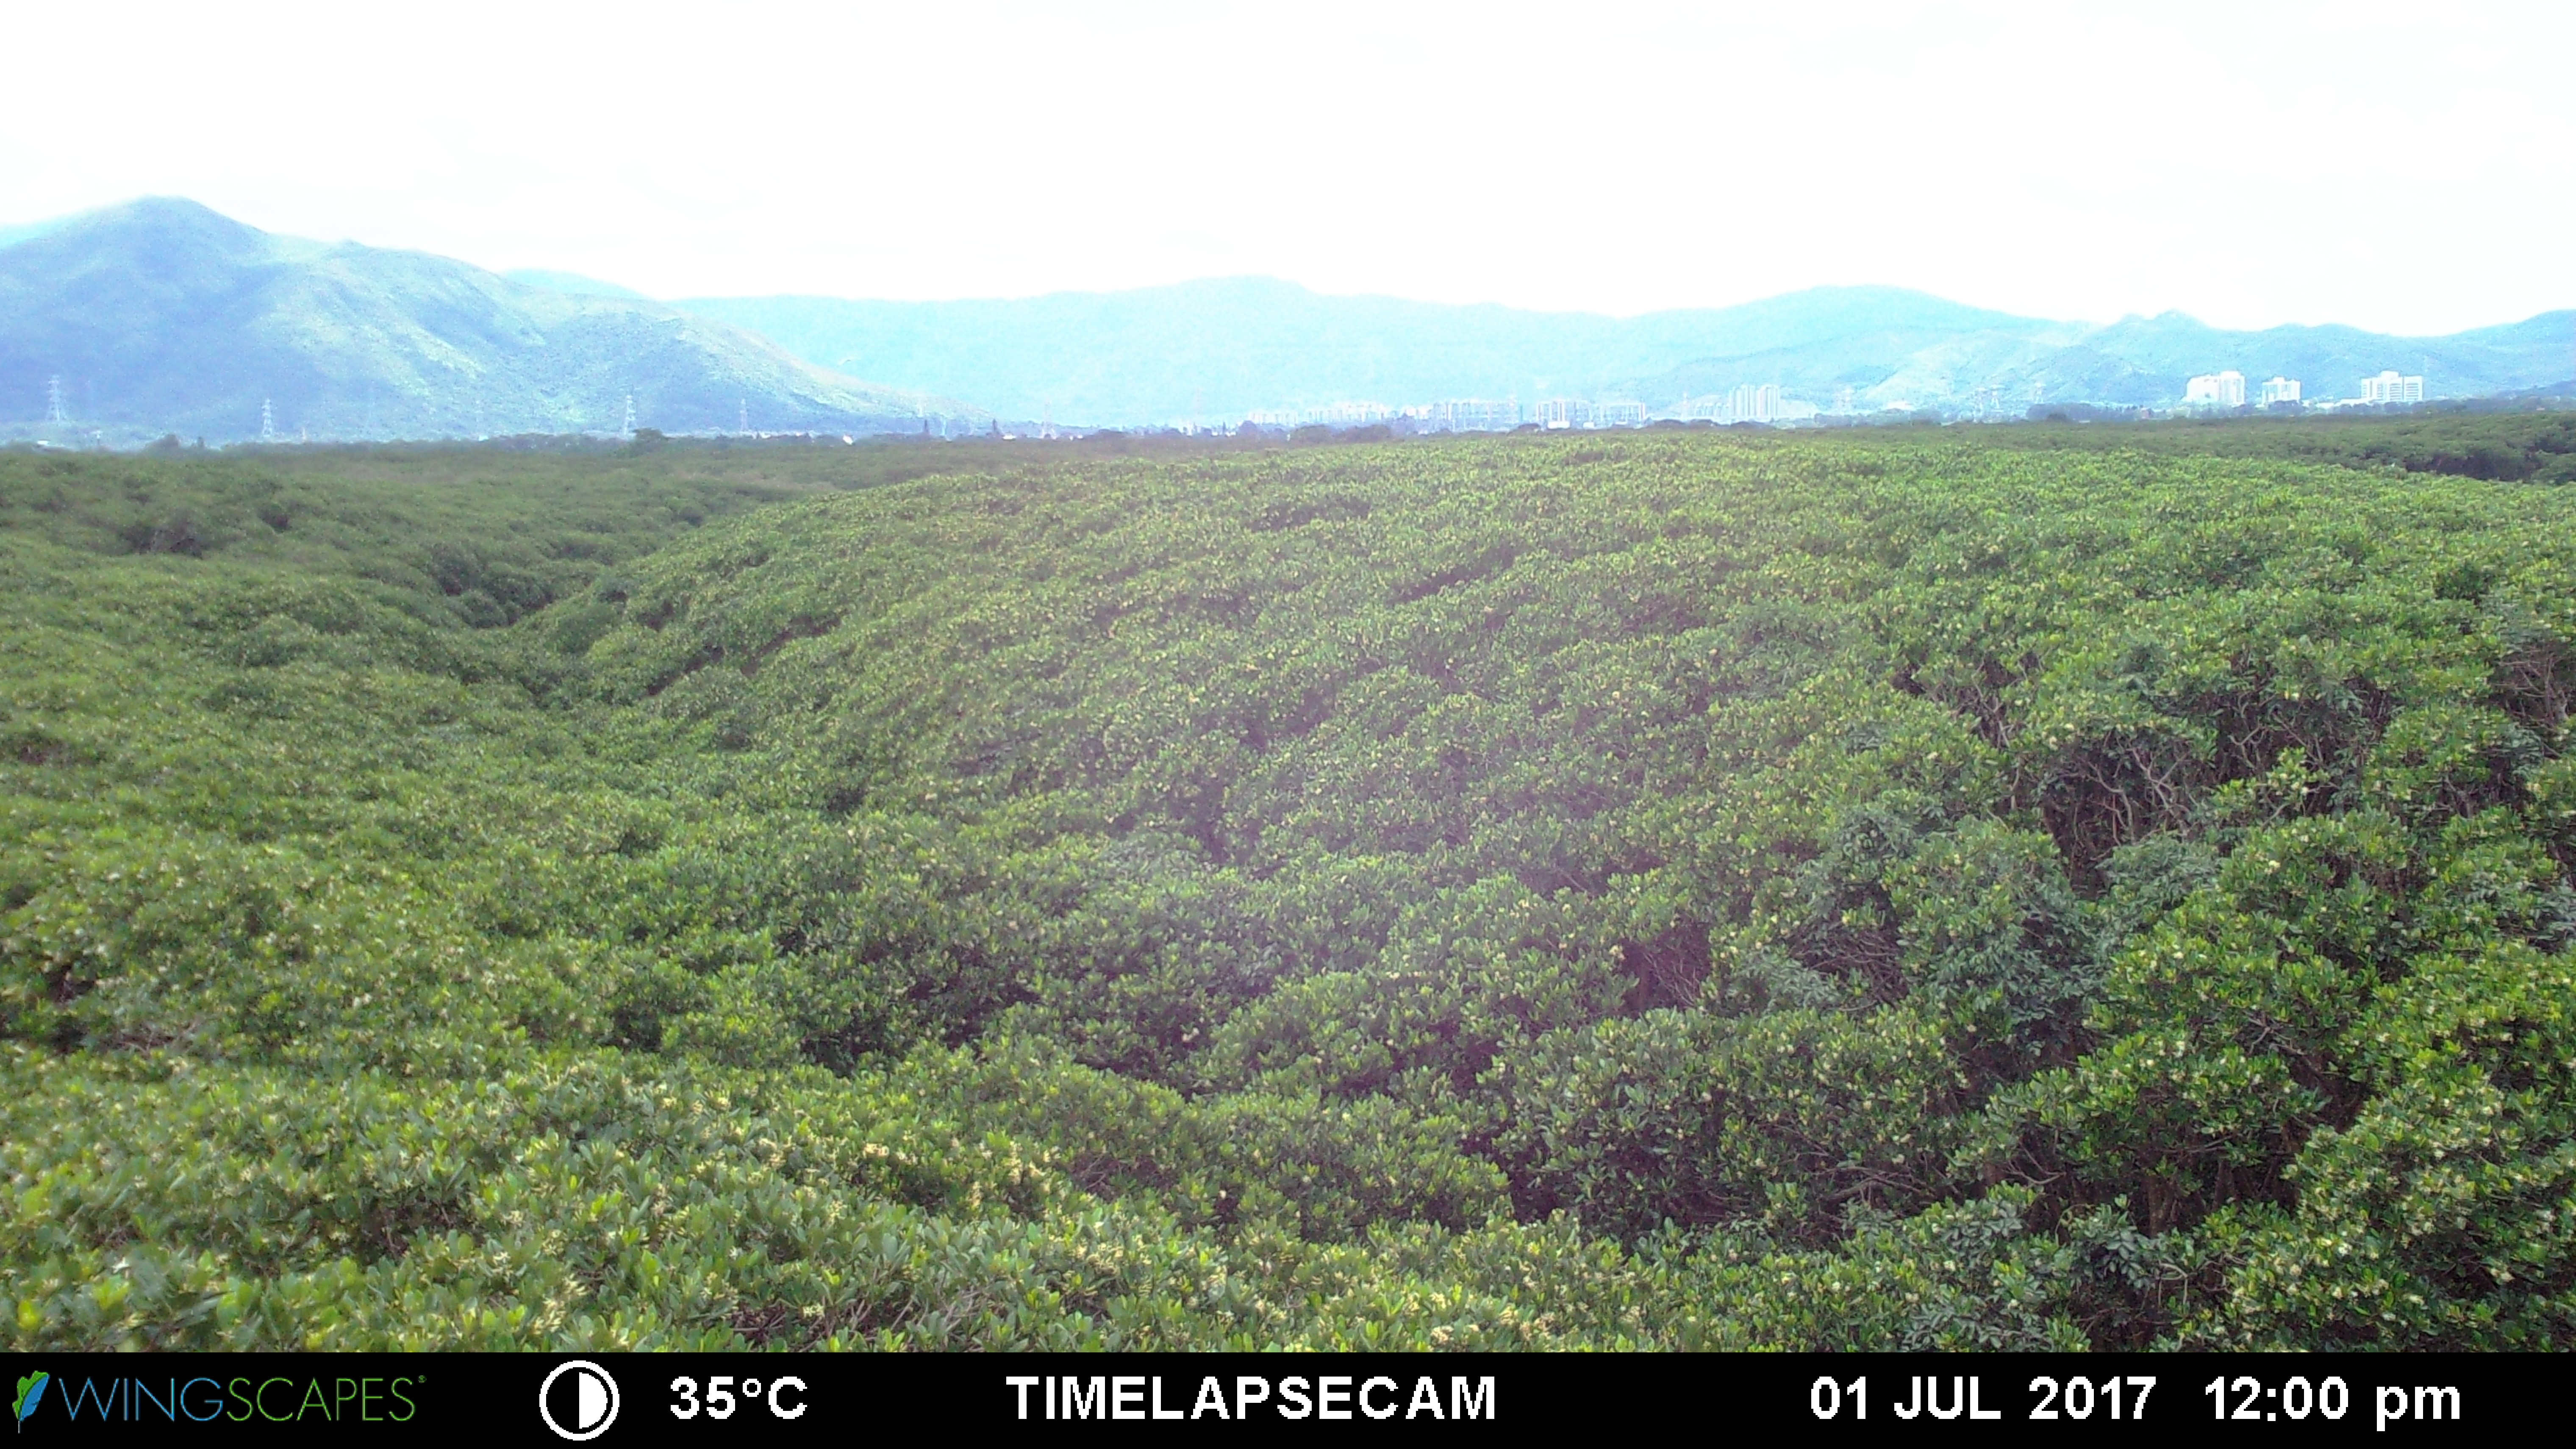
\includegraphics[width=1\textwidth]{pictures/WSCT4349.jpg}
  \includegraphics[width=1\textwidth]{pictures/w.jpg}
  \caption{Image Examples}
  \label{fig:fig1}
\end{figure}
++ Study Area


Search for "Latex, formula format" for more information

\subsubsection{Data Quality Control}
\paragraph{Quality control before and during implementation.}
We ensured that all the images were captured by the same camera on the observation tower.The camera's position and direction were supposed to remain constant all the time during the whole period.We turned automatic aperture and exposure mode on in order to guarantee that among all the images, the illumination conditions stay consistent.


\paragraph{Camera Shifts.}Time series were first visually inspected for camera shifts and the related changes in field of view (FOV). The FOV remained largely unchanged. However, some larger shifts in the FOV were observed as the positioning of the camera changed a few times throughout the study. 

\paragraph{Poor Illumination.}We also observed images with unusual illumination which may affect the calculation of vegetation indices. For example, images before sun rise and after sun set had inadequate illumination and so can hardly be used for monitoring the greenness. Also, images around the sunrise and sunset had significant different hues. 

To wipe out the bad images significantly affected by camera shifting or unusual illumination, we calculated the percentage of green color in each image as an indicator for filtering and calibration. The percentage of green color was computed as the percentage of image pixels where the {DN_g}  was smaller than 175. After applying the greenness proportion calculation to one month’s images, we found that the proportions are segmented to two parts. Irregular images suffering from bad illumination or camera shifting problems had values being extremely close to 1, while the normal ones were normally distributed around 0.6. Therefore, we selected a benchmark of 0.75 to sift out the normal images to be used in further calculations (++ histogram in Supporting Information). Using this filter, we identified and removed XXX images  from the original dataset. Rechecking the identified bad images, we found that they are all ill-illuminated and had a time span from 6pm to the second day’s 6am. See Figure \ref{fig:fig1}.


Moreover, at the bottom of each image, a black bar is attached to display the time, temperature and equipment manufactory, which largely disturbed our calculation of vegetation indices. Noting these noises, images were first cropped to exclude the bars. The way to solve the field of view shifts is discussed in later sections. All image processing were conducted using Python 3.6. 


\subsection{Calculation of Vegetation Indices}
To quantify canopy greenness, we calculated the green chromatic coordinate (GCC), which is widely used to monitor canopy development and is strongly related to GPP (xxxx cite), can be denoted as follows,

\begin{equation}
GCC = \frac{DN_g}{{DN_r + DN_g + DN_b}}
\end{equation}

where the subscripts R, G, and B indicate the red, green, and blue channels, respectively. 
We also computed another vegetation index, the excess green (EXGCC) index, which can be denoted as follows, 

\begin{equation}
EXGCC=2DN(g)-(DN(r)+DN(b)) 
\end{equation}

EXGCC can be less noisy than GCC in some ecosystems, notably in conifer canopies (xxx cite), although GCC is generally more effective than EXGCC in suppressing the effects of changes in scene illumination (xxx cite). Due to the formulas, all the GCCs which are larger than 1 is dropped. All the EXGCCs which are greater than 200 are modified to 200. 


\subsection{Time-Series Smoothing}
Knowing the vegetation indices are sensitive to illumination conditions, we extracted the images ranging from 10am to 2pm during the day to avoid hue changes due to sunset and to have the most stable illumination. We applied a moving window smoothing to the extracted VIs to highlight the underlying monthly and seasonal change patterns by removing several extremities and unexpected fluctuations that appeared in the extracted time series of GCC and EXGCC caused by factors such as slight illumination disturbance, droplets on lens, and cloud. Several smoothing methods including the mean filter, median filter, and 90\% percentile filter were applied for comparison. Following the practice of xxxx (cite), the window size was selected as 3 days. 


\subsection{Validation Methods}
We validate the GCC values extracted (GCCe) from camera photos with field-measurements (GCCf) using the Pearson Correlation Coefficient, and RMSE.    

Pearson Correlation Coefficient: np.corrcoef()
RMSE: 1/ establish a linear transformation from GCCe to GCCf. 2/ estimate the RMSE between GCCe-estimate and GCCf. y = kx + b, RMSE = sigma(yi - yi-hat)**2/N

Exposure Time.  - RMSE 1/ establish a model to predict GCCf with GCCe and Exposure Time. 2/Measure the R2 and RMSE. 


\subsubsection{}



\section{Results} \todo{Finish Section 3.1}

% Figure Requirements: DPI=300




\subsection{Vegetation Indices of Mangroves Extracted from Camera Images}
We calculated the GCC and ExGCC of mangroves for the entire month of July, 2017. Figure \ref{fig:fig1} shows the extracted GCC of mangroves in July,2017 before and after three day mean smoothing.

In summer / winter 

+ Time Series - not smoothed 

We applied three different smoothing method to the extracted time-series of vegetation indices. After analyzing the graphs of three day mean smoothing and three day median smoothing of GCC and ExGCC, We observed that although larger decreases appear on about July 7th and 13th, which were due to rainy weather, the overall curve was stable and had a trend of gradually increasing, as was displayed in Figure \ref{fig:fig1}.


Recognizing the pattern in the VIs series in July, we further generated similar graphs for a entire month of January, 2017, for comparison.
Figure \ref{fig:fig2} shows the extracted GCC of mangroves in July,2017 before and after three day mean smoothing.A large gap between January 14th and January 18th was due to a lost of raw images even before image cleaning.The significant drop was still owing to poor illumination.


When scanning all the images for visible stains, we found that they had different exposure times, which might lead to relatively great or poor illumination conditions.We therefore extracted the exposure times from images' exif datas and compute their correlation  coefficients with GCCs and ExGCCs.Fortunately, we got quite high correlations, about 0.7, between exposure times and VIs in July, which mean we can use exposure times to improve the prediction performances of GCCs and ExGCCs.
\begin{figure}
  \centering
  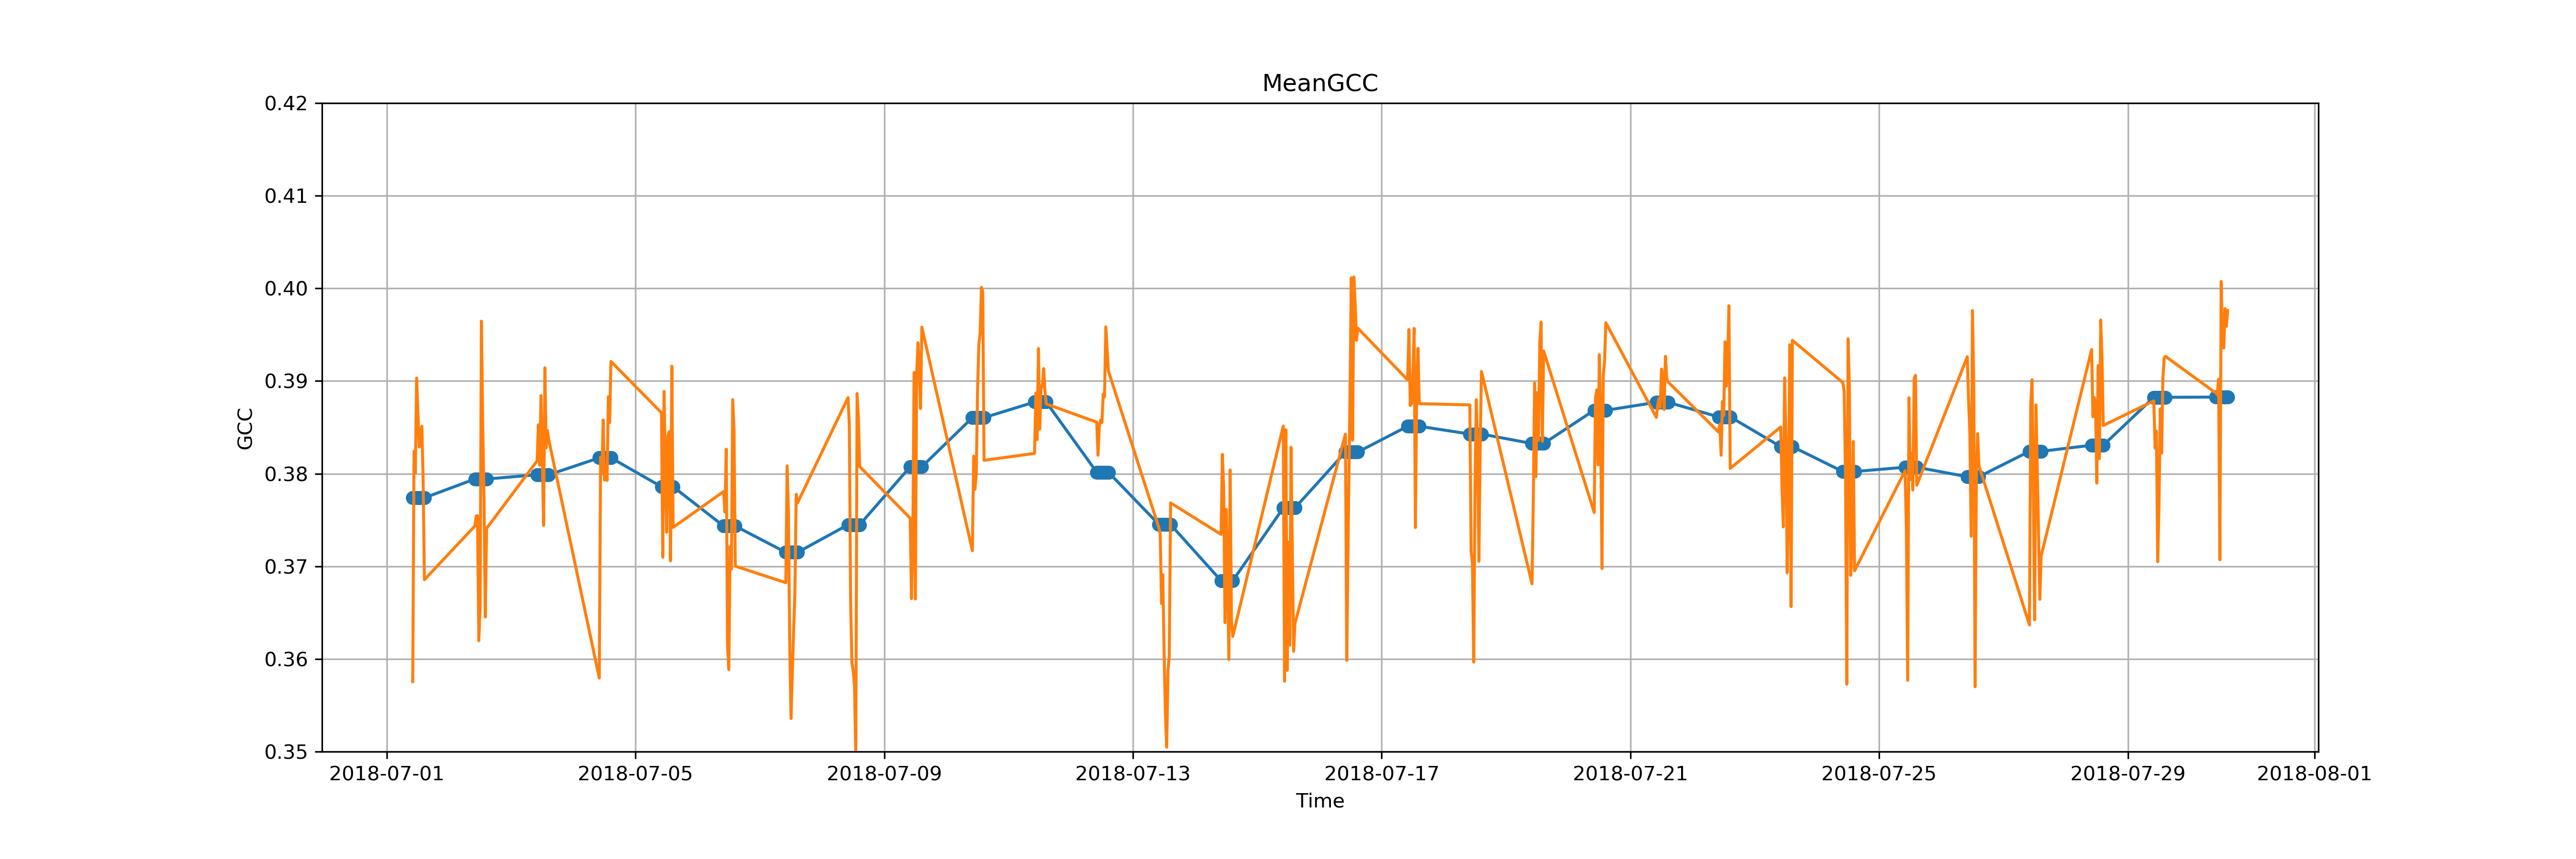
\includegraphics[width=1\textwidth]{pictures/meanGCC.png}
  \caption{Extracted GCC of mangroves in July,2018 before and after three day mean smoothing.}
  \label{fig:fig1}
\end{figure}

\begin{figure}
  \centering
  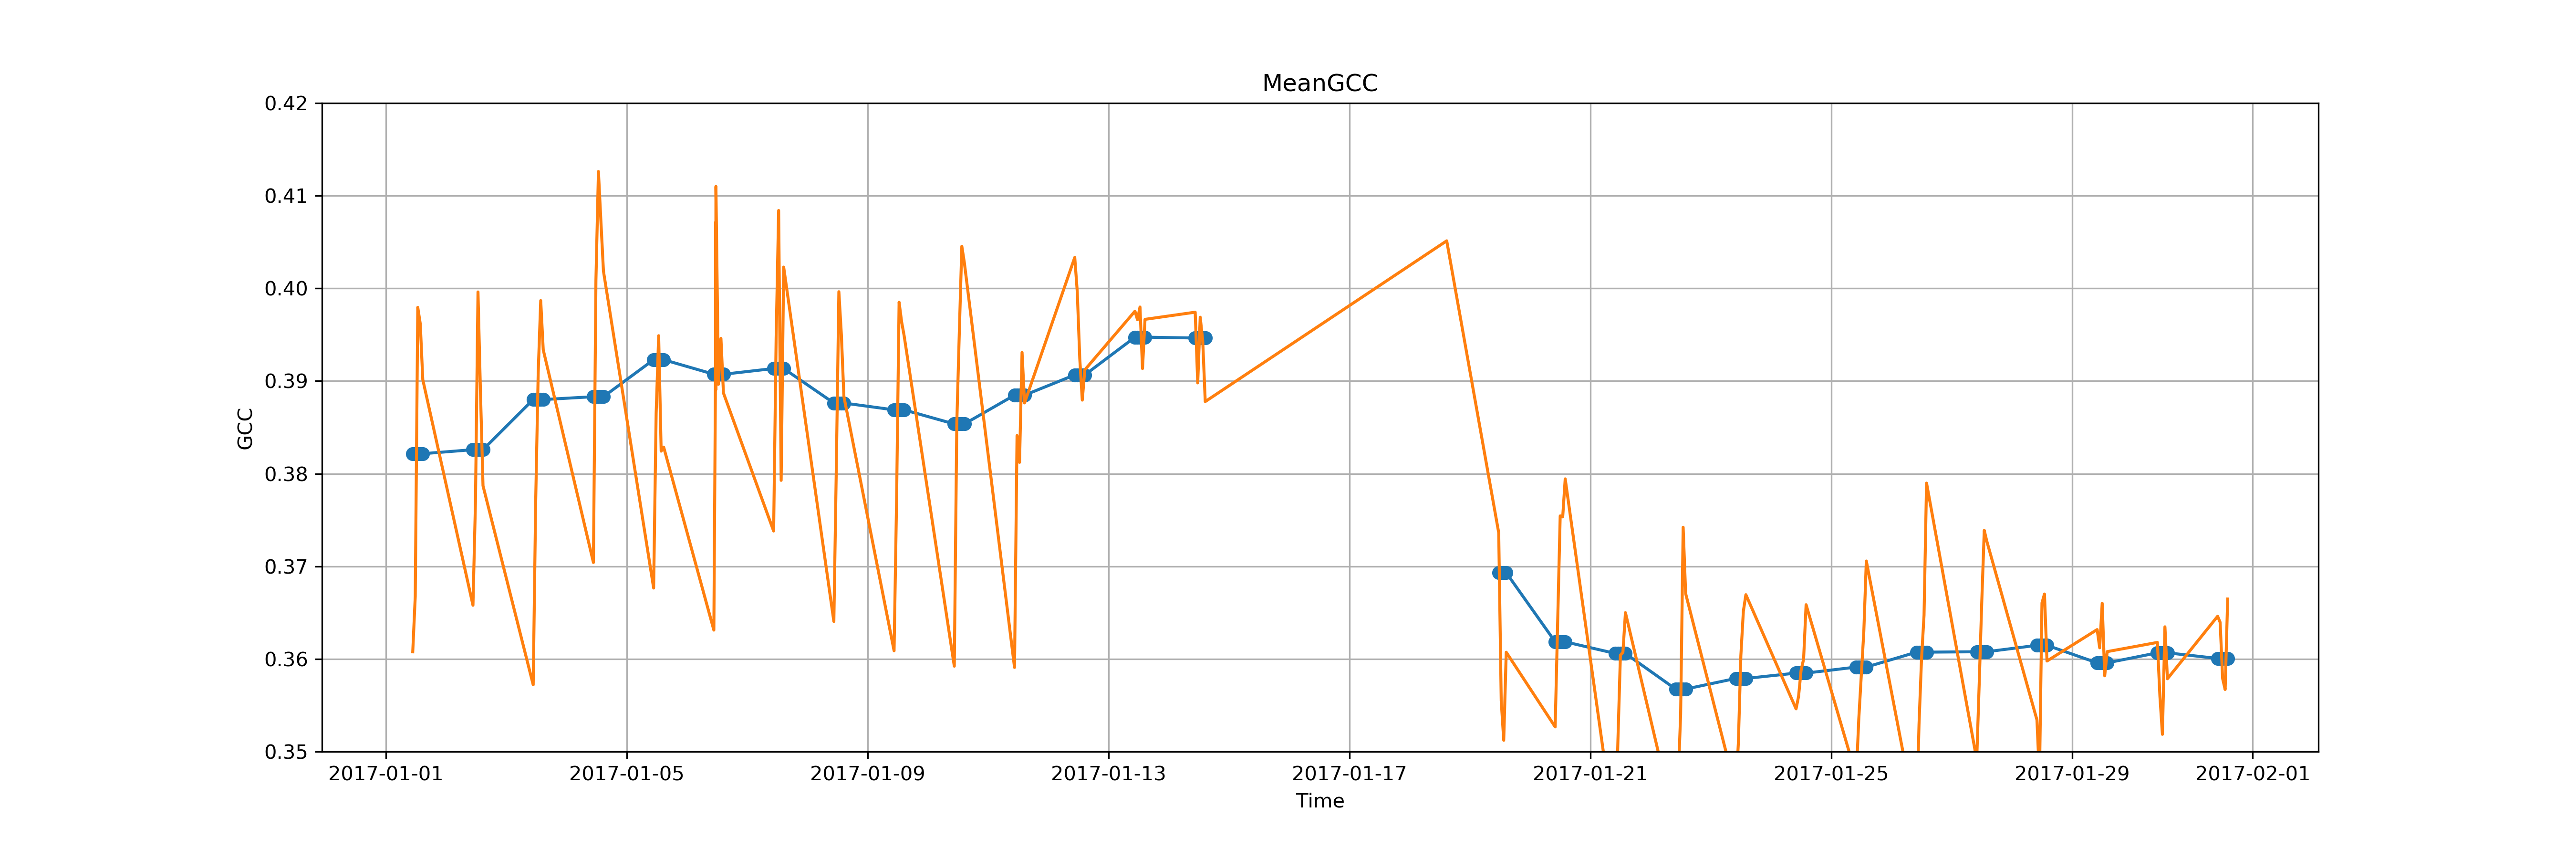
\includegraphics[width=1\textwidth]{pictures/JanmeanGCC.png}
  \caption{Extracted GCC of mangroves in January,2017 before and after three day mean smoothing.}
  \label{fig:fig2}
\end{figure}


\subsection{Validation of the VIs extracted from Camera Photos}

summer 

winter




\section{Discussions} \todo{Finish Section 4.1-4.3}
\subsection{The Pros and Cons of using camera photos to monitor the growth of mangroves}
Digital cameras can produce accurate datas if the VIs can be integrated with other techniques like eddy covariance datas(cite   ).After Comparing it with other methods like landsat datas, we found that we can detect the potential drawbacks of the clear digital images more swiftly and directly and corect them as soon as possible.Using digital images is also a economic research method that it can be used in other scientific cases and save a lot of money if the vegetation indices are representative for one type of environment.

However, the restrictions of digital photos can directly influence the outcome of the research.The location of the cameras should be fixed for such a long time span that it is difficult to ensure the same field of view.
According to our experiment, the VIs and GPP can be not so synchronous due to the change in the illumination condition, the hue of the images and the complexity of the region. 



Uniqueness of Mangroves 

\subsection{The Seasonal Effects}



\subsection{Other Potential Factors that affect the reliability}
\subsubsection{Illumination}
- We observed that the extracted VIs correlate significantly with the illumination conditions. The VIs increases with stronger incoming daylight and decreases with weaker daylight. The change caused by the difference in illumination conditions could even be more dramatic than that caused by the seasonal effects. In this paper, we adopted the method from XXX (2016) and only extracted VIs from images captured from 10am to 2pm when the daylight is relatively stable. Results show that this method helps control the effects of illumination change. 


\subsubsection{Weather effects}
On cloudy days, the gloomy weather largely weakened the illumination due to less incoming sun light.Moreover, the hues displayed on the images were shifted from bright colors to dim and dark ones.These resulted in consequences that some of the days generated extremely low VIs, which had no relationships with the conditions of the mangrove forests.The same situation can be applied to rainy days, which were usually accompanied with clouds.It was noteworthy that on rainy days, large  rain droplets may descent on the lens of the cameras.These stains were also potential causes of sudden decreases in VIs.


\subsubsection{Different smoothing methods}
The moving mean smoothing method generates similar reuslts compared with the moving median smoothing method, while the moving 90\% quantile smoothing method could minimize the fluctuations caused by weather changes and other potential factors.The moving mean smoothing method can be affected by extreme values, which appear relatively frequently in our research.The moving 90\% quantile smoothing method may be inaccurate because it only displays the pattern of datas with large values and so that ignores comparatively small ones.++++ 



\subsection{Other Results for Reference}
\subsubsection{Get Mean First vs. Our Method}



\section{Conclusion}



\bibliographystyle{unsrt}  
%\bibliography{references}  %%% Remove comment to use the external .bib file (using bibtex).
%%% and comment out the ``thebibliography'' section.


%%% Comment out this section when you \bibliography{references} is enabled.
\begin{thebibliography}{1}

\bibitem{kour2014real}
George Kour and Raid Saabne.
\newblock Real-time segmentation of on-line handwritten arabic script.
\newblock In {\em Frontiers in Handwriting Recognition (ICFHR), 2014 14th
  International Conference on}, pages 417--422. IEEE, 2014.

\bibitem{kour2014fast}
George Kour and Raid Saabne.
\newblock Fast classification of handwritten on-line arabic characters.
\newblock In {\em Soft Computing and Pattern Recognition (SoCPaR), 2014 6th
  International Conference of}, pages 312--318. IEEE, 2014.

\bibitem{hadash2018estimate}
Guy Hadash, Einat Kermany, Boaz Carmeli, Ofer Lavi, George Kour, and Alon
  Jacovi.
\newblock Estimate and replace: A novel approach to integrating deep neural
  networks with existing applications.
\newblock {\em arXiv preprint arXiv:1804.09028}, 2018.

\end{thebibliography}


\section{Lecture Notes}

\subsection{May. 4th}
1. [Completed] Compare the get mean first method with the method we used.

We found a minor technical difference between  the extraction method of GCC proposed in existing literature and the method we are using. The difference is that in existing literature GCC was calculated using the averaged grey-level values in the Green, Blue and Red bands, while in our method, we calculate GCC for each pixel based on the RGB value for each pixel first and then average the GCC for each image.

We compared extracted GCC for both methods. The GCC values calculated using our method is slightly larger with a very similar trend. We observed that the GCC extracted using our method has slightly larger variance. However, the advant   age of our method is that for each image we get a distribution of GCC. So it depends on the needs of follow-up studies on the technical procedures.  

+ Comparison Figure


2. Next Steps

2.1 Complete GCC extraction for Feb., 2017.
Outs: 1 .pk file.  2. Curve - before and after smoothing

2.2 Validate the results in Feb.

2.3 Validation results with Exposure Time.  





4. Available Time: AP Exams: May 6/14/15


\end{document}
